\chapter{Introduction to Python}

Python is a general-purpose programming language designed by Guido van Rossum,
with an emphasis on readability and reusability \citep{vanRossum:1996:Foreword}.
It comes with an extensive standard library and is one of the most popular
programming languages.

There are multiple options for interacting with Python, these include:
\begin{itemize}
    \item typing commands into an interpreter,
    \item writing files and running them with an interpreter,
    \item using an online service such as Google Colab.
\end{itemize}
A small snippet of trivial python code is given below to display the syntax.
{\singlespacing
\inputminted[
    frame=lines,
    framesep=2mm,
    mathescape,
    linenos
    ]{python}{Sample.py}
}

\section{Neural Networks in Python}

Before using any neural network packages, a few small examples networks were
produced in python.
The \texttt{numpy} package was used to perform matrix operations,
and the \texttt{matplotlib.pyplot} package was used for plotting,
as these features were non-trivial.
For some examples, the \texttt{keras} module from the \texttt{tensorflow}
package was also used to access specific datasets, but their broader purpose
will be explored in the next section.

\subsection{Single Layer Boston Housing Data}

The first example network consisted of 3 input neurons connected to a
single output neuron, which is given by the equation
\begin{align*}
    y &= \tanh\left(b + \sum_{i=1}^{3} w_ix_i\right).
\end{align*}
The bias term was implemented by adding a forth input node with a constant value
of one, giving
\begin{align*}
    y &= \tanh\left(\mathbf{w}\cdot\mathbf{x}\right),
\end{align*}
where $w_4 = b$, and $x_4 = 1$.

The network was trained using the Boston housing dataset from \texttt{keras},
which provided a number of attributes about houses from late 1970's Boston
suburbs.
The network took in normalised data from three of these attributes (number of
rooms, highway accessibility index, percentage of lower status population), and
used them to predict the value of the house.

Training was performed using backpropagation, defined by the equation
\begin{align*}
    \Delta w_i &= \eta\Rpdiff{e}{w_i},\\
    d &= y - y_t,\\
    e &= \frac{1}{2}d^2,
\end{align*}
where $e$ is the network error, $y$ is the network prediction, and $y_t$ is the
target value.
By definition,
\begin{align*}
    y &= \tanh(\text{net}),\\
    \text{net} &= \sum w_ix_i.
\end{align*}
By chain rule,
\begin{align*}
    \Rpdiff{e}{w_i} &=
    \Rpdiff{e}{y} \cdot \Rpdiff{y}{\text{net}} \cdot \Rpdiff{\text{net}}{w_i}.
    %
    \Rpdiff{net}{w_i} &= x_i,\\
    \Rpdiff{y}{net} &= 1 - \tanh^2(net) = 1 - y^2,\\
    \Rpdiff{e}{y} &= \frac{1}{2}\Rpdiff{(y - y_t)^2}{y} = y - y_t = d,\\
    %
    \therefore\Rpdiff{e}{w_i} &=
    x_i \cdot (1 - y^2) \cdot d.
\end{align*}
$\Delta w_i$ can be written in vector notation, giving
\begin{align*}
    \Delta \mathbf{w} &= \eta\cdot\mathbf{x}\cdot (1-y^2)\cdot d.
\end{align*}
Weights were updated after each sample using
\begin{align*}
    \mathbf{w}' &= \mathbf{w} - \Delta\mathbf{w},
\end{align*}
where $\mathbf{w}'$ is the new set of weights.

The network was initialised using random weights, and was trained using the full
dataset.
\begin{center}
    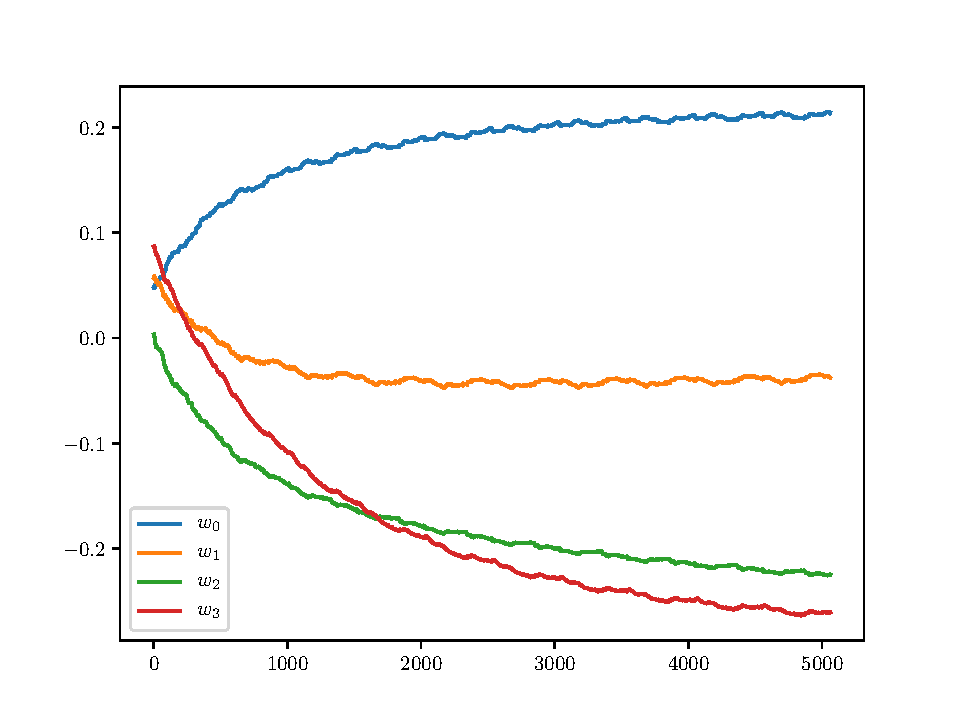
\includegraphics[width=0.7\textwidth]{../Code/BostonHousingResult.pdf}
    \captionof{figure}{Graph of network weights against iteration number.}
\end{center}
After 10 epochs, the mean square error had reduced from 0.1637 to 0.0507.
Note that the weight value lines appear to be jagged, this was a side effect of
updating the value after each individual presentation; a problem which can be
mitigated by batching $\Delta\mathbf{w}$ terms from multiple presentations.



\subsection{Multilayer Boston Housing Data}

The same task was repeated using the full set of attributes.
To accommodate this, a larger network with 13 input neurons, 1 output neuron,
and $n$ hidden neurons; which was expressed by the equation
\begin{align*}
    h_i &= \tanh\left(b_i + \sum_{j=0}^{13} w_{i,j}x_j\right),\\
    y &= b + \sum_{i=1}^{n} w_i h_i.
\end{align*}
Similar to the single layer example, a constant neuron was added to the input
and hidden layer to implement the bias, giving
\begin{align*}
    \mathbf{h} &= \tanh(W\mathbf{x}),\\
    \mathbf{h}' &= \begin{pmatrix} \mathbf{h} \\ 1 \end{pmatrix},\\
    y &= \mathbf{w}\cdot\mathbf{h}',
\end{align*}
where $\tanh$ acts component-wise on the input.

All of the inputs were batched together into a single matrix $X$, where each
column was a data point, giving
\begin{align*}
    \Phi &= \tanh(W\cdot X),\\
    \Psi &= \begin{pmatrix} \Phi \\ \mathbf{1} \end{pmatrix},\\
    \mathbf{y} &= \mathbf{w}\cdot\Psi,
\end{align*}
where $\mathbf{y}$ is a row vector of results.
The error gradients for the output neurons were given by
\begin{align*}
    \mathbf{d} &= \mathbf{y} - \mathbf{y}_t,\\
    e &= \frac{1}{2}\left|\mathbf{d}\right|^2,\\
    \mathbf{g}_O &= \Rpdiff{e}{\mathbf{w}} = \mathbf{d}\cdot\Psi^T;
\end{align*}
and for the hidden neurons by
\begin{align*}
    D &= \hat{\mathbf{w}}^T\cdot\mathbf{d},\\
    G_H &= ((1 - \Phi\odot\Phi)\odot D) \cdot X^T,
\end{align*}
where $\odot$ is the component-wise product, and $\hat{\mathbf{w}}$ is the
weight vector without the bias term.
Note that $\hat{\mathbf{w}}^T$ and $\mathbf{e}$ are column and row vectors
respectively, and that their product is a matrix.
See Appendix \ref{app:BHMDeriv} for full derivation.

\begin{center}
    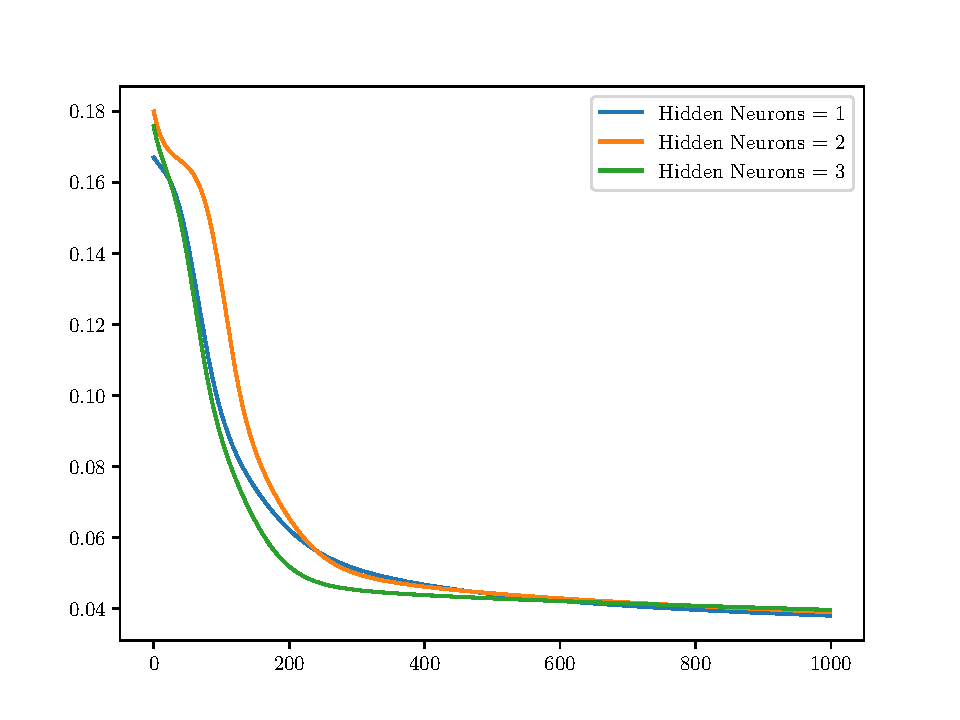
\includegraphics[width=0.7\textwidth]{../Code/BostonHousingMultiResult.pdf}
    \parbox{0.9\textwidth}{%
    \captionof{figure}{Graph of network error against iteration number for
    various numbers of hidden neurons.}}
\end{center}
The network was trained multiple times with varying numbers of hidden neurons.
In each case, the network successfully reduced it's error to roughly the same
level:
for 1 neuron, from 0.1670 to 0.0380;
for 2 neurons, from 0.1799 to 0.0390; and
for 3 neurons, from 0.1757 to 0.0396.
The difference between the results was negligible, which suggested that one
hidden neuron was sufficient for learning the data.

When compared with the single layer network from the previous section, the
single neuron, multilayer network performed better (0.0507 vs 0.0380) for two
reasons:
\begin{enumerate}
    \item it had access to all 13 attributes, instead of the 3 attributes that
        had been manually selected; and
    \item the additional layer enabled it to apply a linear transformation to
        the activation.
\end{enumerate}



\subsection{Logical XOR}

Using the same, multilayer network architecture, a network was trained to
perform the logical exclusive-or operation.

\begin{align*}
    X &= \begin{pmatrix}
        0 & 1 & 0 & 1 \\
        0 & 0 & 1 & 1 \\
        1 & 1 & 1 & 1
    \end{pmatrix},\\
    \mathbf{y} &= \begin{pmatrix}
        0 & 1 & 1 & 0
    \end{pmatrix}.
\end{align*}

\begin{center}
    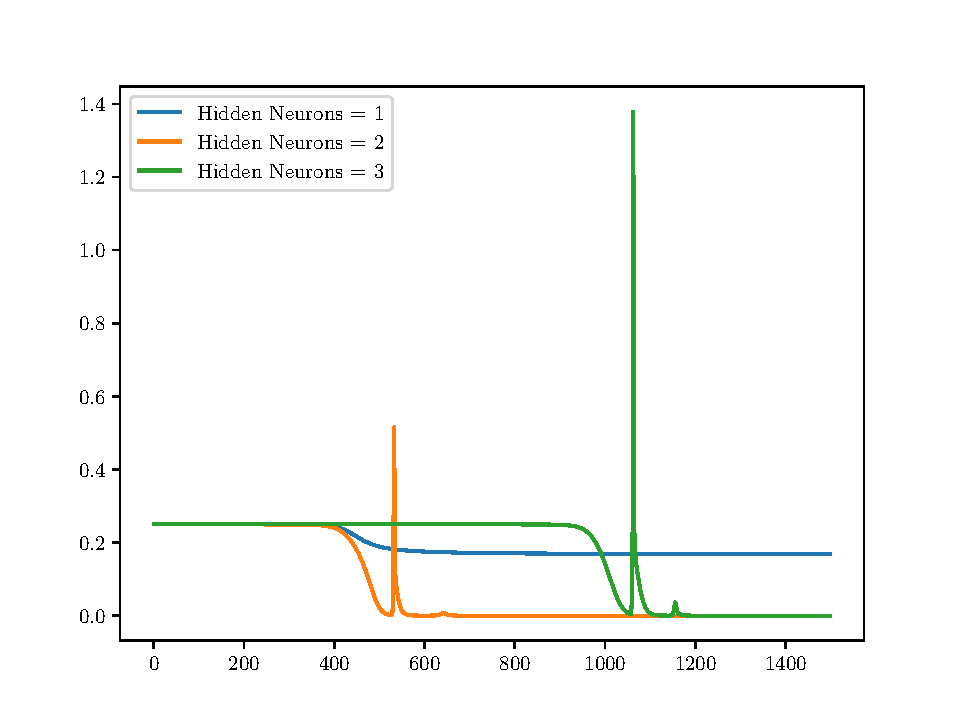
\includegraphics[width=0.7\textwidth]{../Code/XORResult.pdf}
\end{center}

\section{Using TensorFlow and Keras}

\subsection{Boston Housing Data}

\subsection{Logical XOR}

\subsection{Linear Regression}

\subsection{Character Recognition}
